\section{Images Reconstructed by the GAN}
In this section, we begin by discussing phase retrieval using hyperparameters, as mentioned earlier, followed by an analysis in which multiple sources are trained simultaneously. The best performance for image reconstruction has been observed with a learning rate of \(2 \cdot 10^{-4}\), a kernel size of 5×5, and equal noise percentages applied to both the original and generated images. A batch size of 1 is used, and equal training is provided to both the Discriminator and the Generator.

\subsection{Predicted Image from the Trained GAN}
Fig.~\ref{fig:GAN} demonstrates the success of the GAN in training a model for Intensity Interferometry (II) to reconstruct images of fast-rotating stars. The GAN was trained on the training datasets for 60,000 steps and subsequently tested on various validation datasets to produce predicted images of a fast-rotating star. In Fig.~\ref{fig:GAN}, four combined images illustrate the GAN's performance in reconstructing the star’s shape, size, and brightness distribution using II.
\begin{itemize}
\item{The left panel shows the signals collected from six baselines, which serve as the input for the Generator during training.}
\item{The first middle panel displays the real image, or ground truth, which the Discriminator uses to distinguish between real images and those generated by the Generator. During training, the GAN aims to replicate these ground truth images.}
\item{The second middle panel presents the reconstructed, or predicted, image produced by the trained GAN, highlighting its success in image reconstruction.}
\item{The right panel shows the difference between the ground truth and the predicted image, with a smaller difference indicating higher precision in image reconstruction.}
\end{itemize}
The predicted images in Fig.~\ref{fig:GAN} yield encouraging results, accurately conveying visual information about the source's size, shape, and brightness distribution across its surface using only six baselines. However, further improvements can be achieved by increasing the number of telescopes to maximize coverage of the $(u, v)$ plane, making the existing and upcoming CTAO an ideal candidate for this approach.

\begin{figure*}
	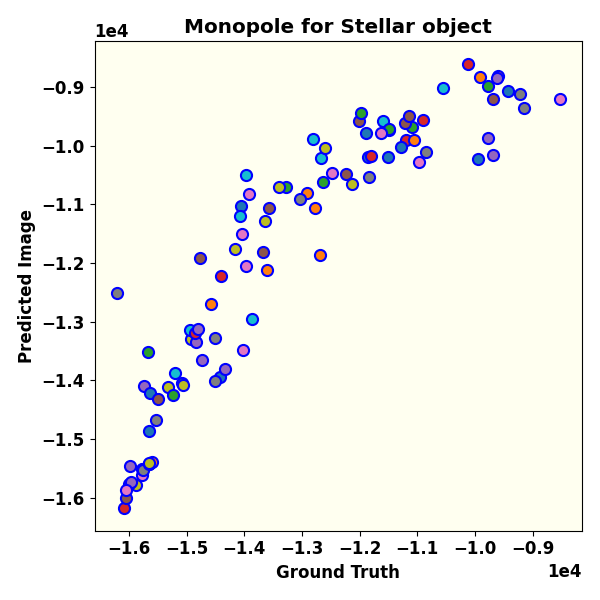
\includegraphics[width=.32\linewidth]{fig/moments/mom0.png}\hfil
	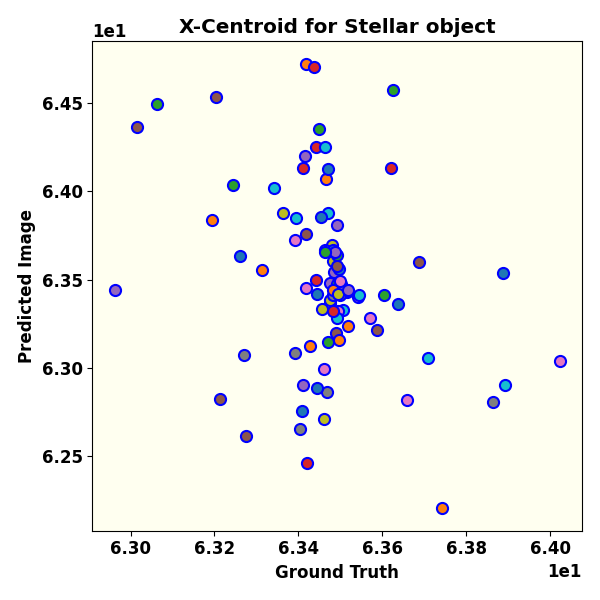
\includegraphics[width=.32\linewidth]{fig/moments/mom1.png}\hfil
	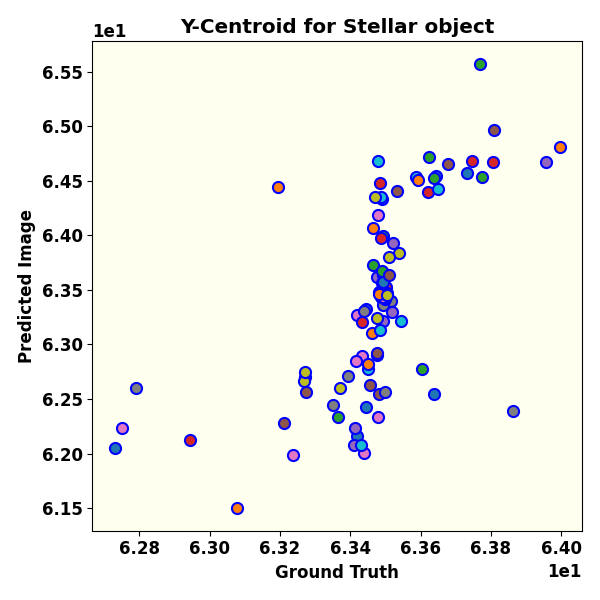
\includegraphics[width=.32\linewidth]{fig/moments/mom2.png}\hfil
	\caption{This set of figures shows the comparison of monopole, x-centroid, and y-centroid for ground truth and predicted images generated by trained GAN.}
	\label{fig:cen}
\end{figure*}
\subsection{Evaluation of GAN using Moments}
The reconstructed images are visually compelling, demonstrating the GAN's effectiveness in using II to reconstruct images. However, visual assessment alone is insufficient; statistical evaluation is necessary to validate the results. To achieve this, we employ image moments as a statistical method. Image moments capture key properties of the reconstructed objects—such as shape, size, and intensity distribution—by quantifying features like position, orientation, and brightness distribution. By comparing the moments of the GAN-generated images to those of the ground truth, we can objectively assess the consistency and accuracy of the reconstruction. This approach provides a reliable framework for evaluating reconstruction quality, as image moments can reveal subtle differences in geometric and intensity properties that might not be apparent through visual inspection alone.

The raw moment $M_{ij}$ of an image $I(x, y)$ is defined as \citep{hu1962visual}
\begin{equation}
	M_{ij} = \sum_{x} \sum_{y} x^i y^j I(x, y).
	\label{eqn:Mom}
\end{equation}
The zeroth order raw moment, or monopole, represents the total intensity of an image. It is computed by summing all pixel values across the image, yielding an overall intensity measure. In this context, analyzing the monopole provides the total flux of fast-rotating stars. According to Eq.~\eqref{eqn:Mom}, the monopole of an image is calculated as:
\begin{equation}
	M_{00} = \sum_{x} \sum_{y} I(x, y).
\end{equation}
The left figure of Fig.~\ref{fig:cen} displays the monopole values for 50 reconstructed images. The plot reveals a linear relationship between the monopole of the ground truth (real image) on the $x$-axis and that of the predicted (reconstructed) image on the $y$-axis, consistent across sources of varying shapes and sizes. This linearity confirms that the predicted images have an overall intensity (flux) that closely matches the ground truth. However, while the monopole effectively represents the total brightness, it does not provide information about the position, shape, size, or detailed brightness distribution of the fast-rotating stars. For these aspects, higher-order moments are necessary.

The center of mass for the fast-rotating star or any other stellar object is calculated using the centroid ($x$-centroid and $y$-centroid). It represents the spatial position of the image and is calculated using first-order raw moment and monopole. The formulation of centroid along the $x$ and $y$ directions is
\begin{equation}
	\begin{aligned}
		&m_x = \frac{\sum_{x} x I(x,y)}{\sum_{x} \sum_{y} I(x, y)} = \frac{M_{10}}{M_{00}} \\
		&m_y = \frac{\sum_{y} y I(x,y)}{\sum_{x} \sum_{y} I(x, y)} = \frac{M_{01}}{M_{00}}
	\end{aligned}  
\end{equation}
The middle and right figure of Fig.~\ref{fig:cen} show the comparison of the $x$-centroid and $y$-centroid for 50 predicted images with respect to ground truths, respectively. The clustering of centroids in a given scale range for all the results explains that the reconstructed image correctly represents the spatial location of the fast-rotating star compared with the ground truth.

The center of mass of a fast-rotating star, or any stellar object, is determined by its centroid, which provides the $x$ and $y$ coordinates representing the spatial position of the image. This centroid is computed using the first-order raw moments in conjunction with the monopole (the zeroth-order moment). The formulations for the centroid along the $x$ and $y$ directions are given by:
\begin{eqnarray}
&&x_c = \frac{M_{10}}{M_{00}} = \frac{\sum_{x,y} x \cdot I(x,y)}{\sum_{x,y} I(x,y)} \nonumber \\
&&y_c = \frac{M_{01}}{M_{00}} = \frac{\sum_{x,y} y \cdot I(x,y)}{\sum_{x,y} I(x,y)}
\end{eqnarray}
Here, \(I(x,y)\) represents the intensity at pixel \((x,y)\), \(M_{00}\) is the monopole (total intensity), and \(M_{10}\) and \(M_{01}\) are the first-order raw moments along the $x$ and $y$ axes, respectively. This formulation accurately captures the spatial center of mass of the stellar object in the image.

The middle and right panel of Fig.~\ref{fig:cen} compare the centroids ($x_{c}$, $y_{c}$) of 50 predicted images with their corresponding ground truths, respectively. The clustering of centroids within a specific scale range across all results indicates that the reconstructed images accurately represent the spatial location of the fast-rotating star relative to the ground truth.

\begin{figure*}
  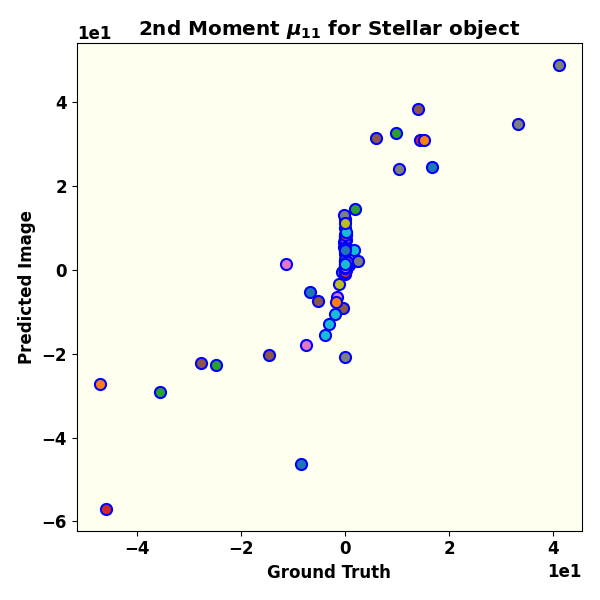
\includegraphics[width=.32\linewidth]{fig/moments/mom3.png}\hfil
  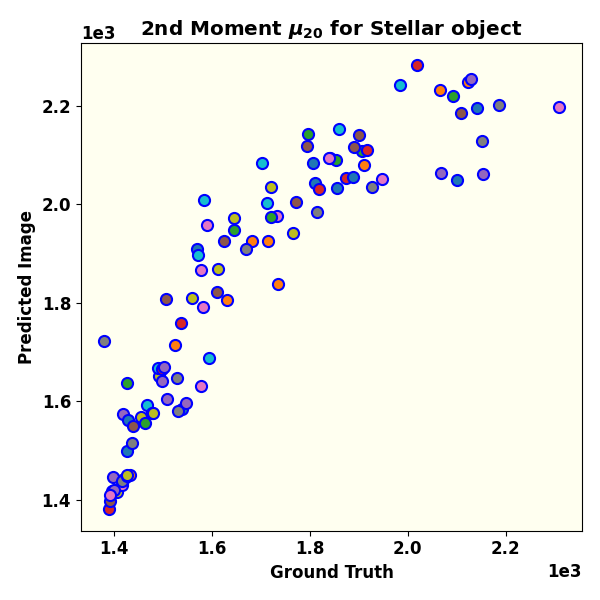
\includegraphics[width=.32\linewidth]{fig/moments/mom4.png}\hfil
  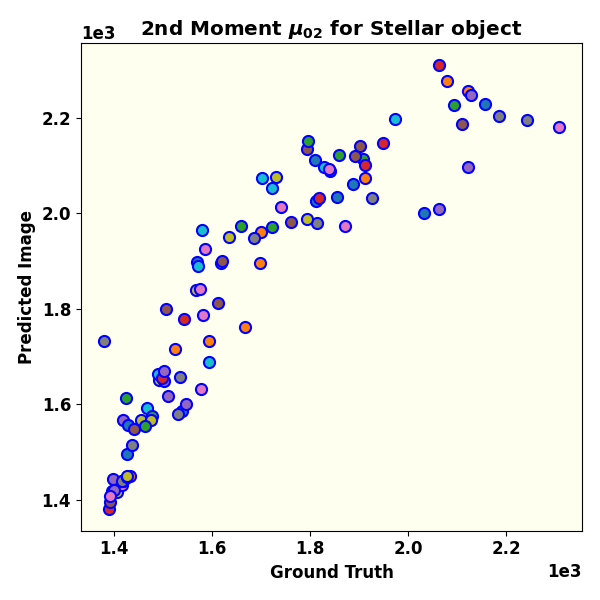
\includegraphics[width=.32\linewidth]{fig/moments/mom5.png}\hfil
  \caption{The second-order central moments provide information about the size and shape of stellar objects.  Shown here are all the second-order central moments for ground truth and predicted images generated by the trained GAN. From left to right these are $\mu_{11},\mu_{20},\mu_{02}$.}
	\label{fig:struc}
\end{figure*}
\begin{figure*}
  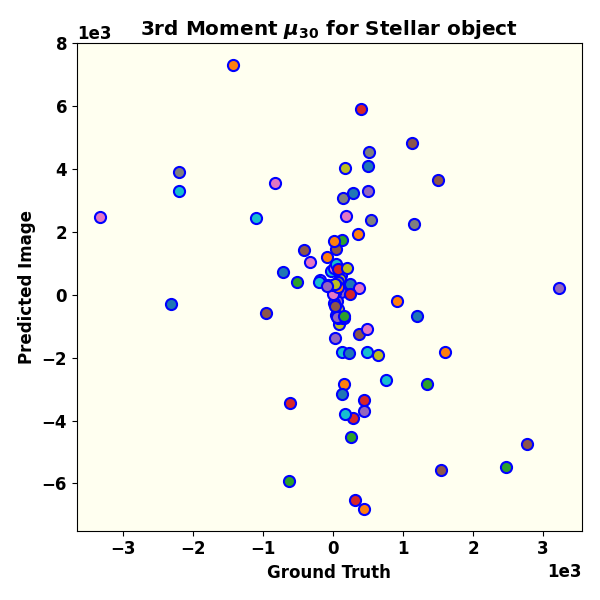
\includegraphics[width=.49\linewidth]{fig/moments/mom6.png}\hfil
  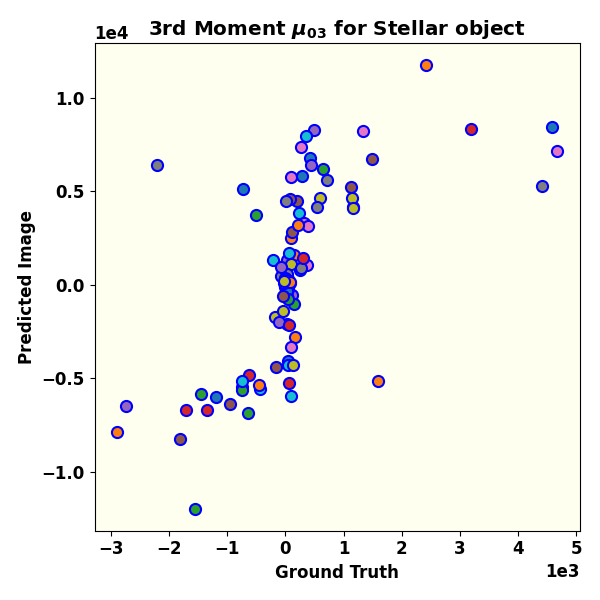
\includegraphics[width=.49\linewidth]{fig/moments/mom7.png}\hfil
  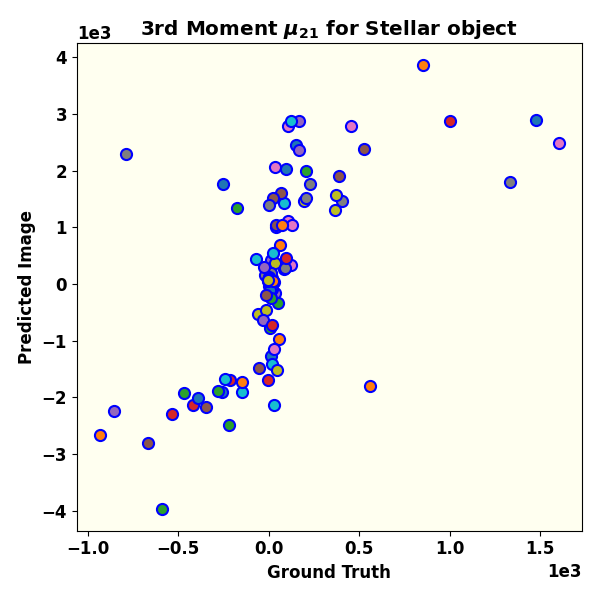
\includegraphics[width=.49\linewidth]{fig/moments/mom8.png}\hfil
  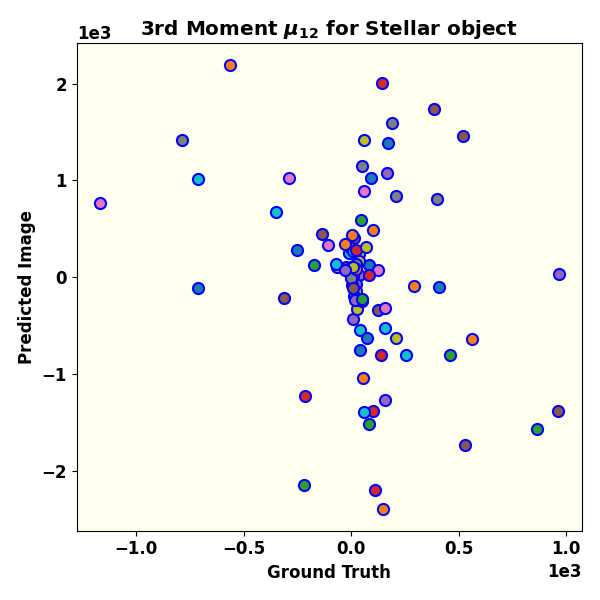
\includegraphics[width=.49\linewidth]{fig/moments/mom9.png}\hfil
  \caption{Shown here are all the third-order central moments for
    ground truth and predicted images generated by the trained GAN.
    They represent the skewness of the brightness distributions.  The
    panels in reading order show
    $\mu_{30},\mu_{03},\mu_{21},\mu_{12}$.}
  \label{fig:moments}
\end{figure*}
%%%%%%%%%%%%%%%%%%%%%%%%%%%%%%%%%%%%%%%%%%%%
Furthermore, these calculated centroids are instrumental in analyzing the shape, size, and brightness distribution of fast-rotating stars using higher-order image moments. To this end, the central moment of an image is calculated according to:
\begin{equation}
	\mu_{pq} = \frac{1}{M_{00}}\sum_{x} \sum_{y} (x - x_c)^p (y - y_c)^q I(x, y).
\end{equation}
The sum of \(p\) and \(q\) defines the order of the central moment. 

Fig.~\ref{fig:struc} presents the second-order central moments (\(\mu_{11}, \mu_{20}, \mu_{02}\)), which are used to study the structure of a fast-rotating star along the line of sight (as explained in the upcoming subsection). All three plots demonstrate a linear relationship in the second-order moments, similar to the monopole, thereby confirming the success of applying the GAN to reconstruct images with II.

The brightness distribution is characterized by the skewness of the image, which is quantified by calculating the third-order central moments (\(\mu_{30}, \mu_{03}, \mu_{21}, \mu_{12}\)). Fig.~\ref{fig:moments} presents all third-order moments for both the ground truth and the reconstructed image. The skewness along the $x$ and $y$ axes (\(\mu_{30}\) and \(\mu_{03}\)) appears acceptable, as shown in both upper panel of Fig.~\ref{fig:moments}, where a linear relationship exists between the ground truth and predicted images. However, the other higher-order moments (\(\mu_{21}\) and \(\mu_{12}\))—particularly \(\mu_{12}\), as depicted in both lower panel of Fig.~\ref{fig:moments}—do not align as well. This indicates that further improvement is possible and should be investigated.

\subsection{The reconstructed Parameters for object}
The centroids \((x_c, y_c)\) indicate only the center of the fast-rotating star and its spatial location in the image. In contrast, the second-order central moments determine the orientation, semi-major axis, and eccentricity relative to the source's center \citep{teague1980image}. These moment-based parameters fully describe the two-dimensional ellipse that fits the image data.

The orientation of a fast-rotating star along the line of sight is defined in terms of second-order central moments as
\begin{equation}
	\theta = \tfrac{1}{2}\arctan \left(\frac{2\mu_{11}}{\mu_{20} - \mu_{02}}\right).
	\label{eqn:orn}
\end{equation}
The semi-major and semi-minor axes of the stellar object are computed using the second-order central moments and are denoted as \(a\) and \(b\), respectively.
\begin{equation}
	\begin{aligned}
		&a = 2\sqrt{mp + \delta} \\
		&b = 2\sqrt{mp - \delta}
	\end{aligned}
	\label{eqn:semi}
\end{equation}
where,
\begin{equation}
	mp = \frac{\mu_{20} + \mu_{02}}{2}
	\label{eqn:mp}
\end{equation}
and
\begin{equation}
	\delta = \frac{\sqrt{4\mu_{11}^2 + (\mu_{20} - \mu_{02})^2}}{2}.	
	\label{eqn:delta}
\end{equation}
Using the calculated axis values, the eccentricity of the fast-rotating star is determined as:
\begin{equation}
	e = \sqrt{1 - a/b}.
	\label{eqn:eccen}
\end{equation}
Eqs.~\ref{eqn:orn}-\ref{eqn:eccen} describe the elliptical nature of the stellar object (in this case, a fast-rotating star) and provide information on its shape and size, depending on the computed values. In contrast, the brightness distribution is characterized by skewness, which is quantified using third and higher-order moments.
